%%%%%%%%%%%%%%%%%%%%%%%%%%%%%%%%%%%%%%%%%%%%%%%%%%%%%%%%%%%%%%%%%%%%%%%%%%%%%%%
% CAPÍTULO 4

\chapter{ASPECTOS GERAIS DAS TÉCNICAS UTILIZADAS}
\label{caputiltecnicas}

Neste capítulo é feita uma descrição detalhada dos métodos e dos algoritmos disponíveis para a caracterização de caos determinístico presente em séries temporais experimentais. Tal descrição será focada nos procedimentos mais utilizados para a reconstrução da dinâmica, para o cálculo de dimensão de atratores e do espectro de expoentes de Lyapunov. São abordados alguns problemas e limitações, do ponto de vista numérico, associados aos algoritmos utilizados, como também as dificuldades encontradas no tratamento de sinais experimentais. 

\section{Caos em séries temporais}

\subsection{Introdução}

\citeonline{alligood/97} afirmam que ``Obviamente, a idéia de que um experimento real possa ser governado por um conjunto de equações é uma ficção. Um conjunto de equações diferenciais, ou um mapa, pode modelar um sistema apenas de forma o suficiente para fornecer resultados úteis''. Por outro lado, a informação completa de todos os graus de liberdade de um sistema dinâmico complexo na natureza é raramente conhecida em sua totalidade. Por exemplo, em um fluido, esta informação deveria incluir sua velocidade em todas as posições como função do tempo, o que é inviável na prática. Neste contexto, torna-se importante analisar sistemas dinâmicos sem que se conheça detalhes sobre a sua dinâmica interna, ou seja, sistemas que não possuem um modelo matemático estabelecido. Uma alternativa para isso é a análise de séries temporais que podem ser obtidas diretamente a partir de um experimento~\cite{kantz/97}.

De uma maneira geral, em um experimento monitora-se uma única variável do sistema, que se sabe de antemão depender das outras. Ou seja, obtém-se uma série temporal de medidas e, na maioria dos casos, não se tem acesso às outras variáveis relevantes (muitas vezes não se sabe ao certo sequer quantas são) e muito menos se dispõe de um modelo (equações diferenciais ou mapas) que descreva o comportamento do sistema. Caso se soubesse exatamente quais são as variáveis relevantes e as mesmas pudessem ser medidas simultaneamente, poderia ser construído um espaço de fase do sistema e nele representar a dinâmica do sistema~\cite{aguirre/00}.

Nesta seção apresenta-se, de maneira geral, um resumo de diversas técnicas utilizadas na identificação de séries temporais caóticas, discutem-se suas principais limitações e enumeram-se quais informações pode-se extrair de sinais experimentais através desses procedimentos. Sempre que possível, tais técnicas serão validadas a partir de uma série temporal que apresenta comportamento caótico, a saber, a componente $x$ do sistema de Lorenz, que foi obtida a partir da solução numérica do Sistema~(\ref{eqsistemalorenzpart}) pelo método de Runge-Kutta de quarta ordem.

\subsection{A Análise Tradicional de Sinais Experimentais}
\label{secanalisetrad}

A identificação de processos regulares pode ser feita através do uso de métodos clássicos. Incluem-se entre eles: a \textit{análise espectral} (espectro de potências) e a \textit{função de autocorrelação}, os quais serão introduzidos a seguir.

Seja a evolução de um sistema dinâmico dada por uma função $f(t)$, ou, quando resultado de uma série de medidas realizadas a intervalos de tempos regulares $\Delta t$, representada por uma série temporal da forma

\begin{equation}
{x_{n}}=x(t_{n}), \;\;\;\; t_{n}=n\Delta t
\label{eqserietemp}
\end{equation}

Sob condições bem gerais, uma função $f(t)$ pode ser considerada como sendo a superposição de um número (eventualmente infinito) de componentes periódicas. A determinação do peso relativo de cada uma dessas componentes é chamada de \textit{análise espectral}. Se $f(t)$ é periódica, seu espectro pode ser representado como a combinação linear de oscilações cujas freqüências são múltiplos inteiros da freqüência básica $\omega$. Essa combinação linear é chamada \textit{série de Fourier}~\cite{papoulis/62}. Quando $f(t)$ é não-periódica, o espectro de freqüências varia continuamente e usa-se a chamada \textit{transformada de Fourier} para representar $f(t)$ em termos dessas freqüências~\cite{papoulis/62}. Escreve-se a transformada de Fourier de $f(t)$ como
\begin{equation}
f(\omega)=\int_{-\infty}^{+\infty}e^{-i\omega t}f(t)dt
\label{eqfouriercont}
\end{equation} 

O espectro de potências $P(\omega)$, que indica o ``peso relativo'' com que a freqüência $\omega$ comparece na composição de $f(t)$, é definido como o quadrado do módulo de $f(\omega)$, ou seja,
\begin{equation}
P(\omega)=\left|f(\omega)\right|^2
\label{eqespectrocont}
\end{equation} 

Na situação de interesse prático, dispõe-se de uma série temporal finita e discreta da forma~(\ref{eqserietemp}). Se $N$ é o número total de pontos na série, então ${x_{n}}$ corresponde a um tempo total de medida $t_\textrm{max}=N\Delta t$. A transformada discreta de Fourier, de uma série temporal, é definida por uma outra série $\widehat{x}_{k}$ tal que
\begin{equation}
\widehat{x}_{k}=\frac{1}{\sqrt{N}}\sum_{n=1}^{N}x_{n}\exp\left[i\frac{2\pi nk}{N}\right],\;\;\;\;\;\;\;k=1.\ldots,N
\label{eqfourierdis}
\end{equation} 

A série temporal~(\ref{eqserietemp}) depende do tempo; por outro lado, $\widehat{x}_{k}$ depende das freqüências, isto é, $\widehat{x}_{k}=\widehat{x}(\omega=k\Delta f)$ com $\Delta f= 1/t_{\textrm{max}}$. O cálculo da transformada discreta de Fourier (\ref{eqfourierdis}) pode ser feito com rapidez através do uso do algoritmo conhecido como FFT (\textit{Fast Fourier Transform})~\cite{cooleytukey/65}.

O espectro de potências $P(\omega)$ para uma série temporal discreta é definido por
\begin{equation}
P(\omega)=\left|\widehat{x}_{k}\right|^2
\label{eqespectrodiscr}
\end{equation} 

Séries temporais com evoluções diferentes apresentam diferentes espectros de potência. Sinais periódicos de período $T$ apresentam um pico bem definido na freqüência correspondente a esse período. Por outro lado, séries temporais caóticas apresentam espectros de potência com uma ``banda larga'', o que indica a existência de um contínuo de freqüências. Séries aperiódicas sem comportamento caótico também podem apresentar um espectro de potência com uma banda larga, e desta forma, é necessário outras ferramentas para caracterizar comportamento caótico em séries temporais~\cite{tufillaro/92}. 

A Figura~\ref{lorenzespec}(b) apresenta o espectro de potências associado à variável $x$, que é parte da solução do Sistema~(\ref{eqsistemalorenzpart}). Pode-se observar que esse espectro apresenta uma ``banda larga'', o que indica a existência de um contínuo de freqüências. Este comportamento é necessário, mas não suficiente para a caracterização de uma dinâmica caótica na série temporal em estudo.

%aperiódicas apresentam espectros de potência contínuos (ver Figura~\ref{lorenzespec}(b)). Portanto, um \textit{espectro de potências contínuo} pode definir uma série temporal caótica, como também um processo aleatório. 

\begin{figure}[ht]
\centering 
\resizebox{7.2cm}{!}{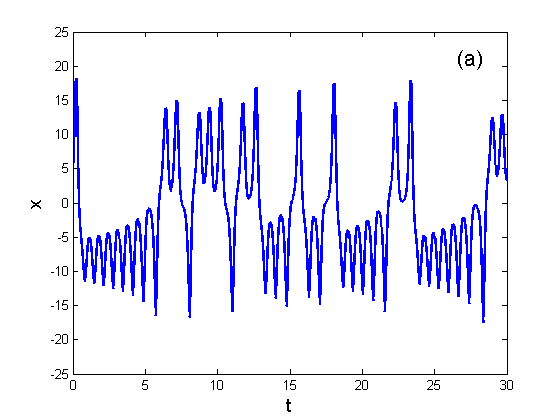
\includegraphics{Figuras/lorenzst.png}} \resizebox{7.2cm}{!}{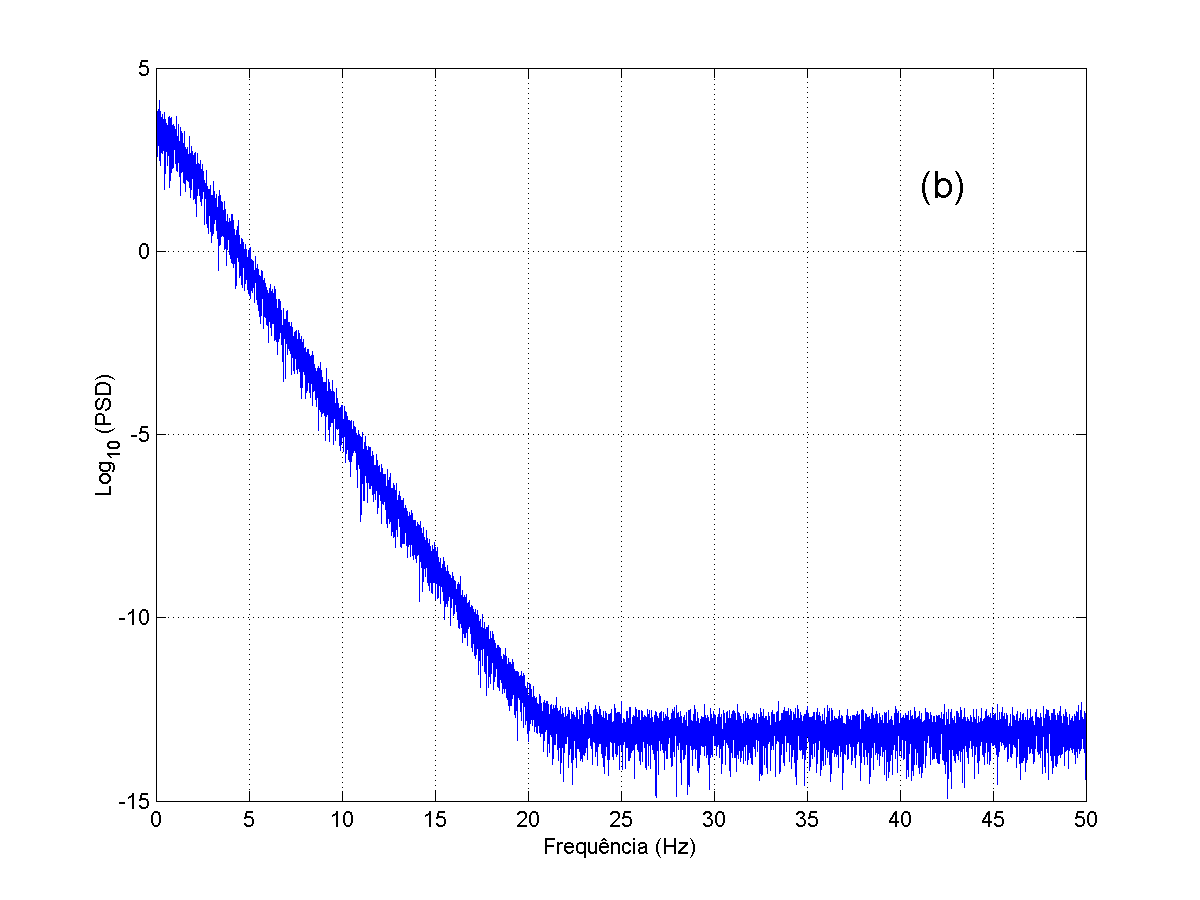
\includegraphics{Figuras/lorenzespectrogrid.png}} \\  \resizebox{7.2cm}{!}{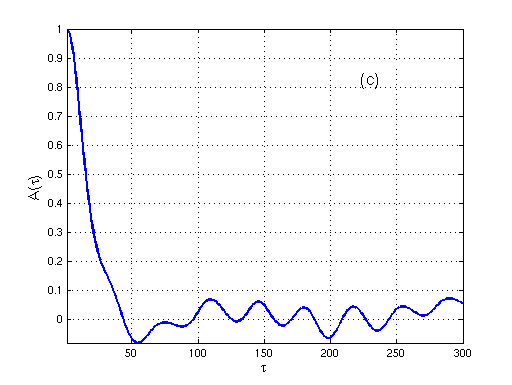
\includegraphics{Figuras/lorenzautocorrgrid.png}} 
\caption{(a) Série temporal caótica da variável $x$ que é parte da solução do sistema~(\ref{eqsistemalorenzpart}). (b) Espectro de potência para a série temporal representada em (a). (c) Função de autocorrelação para a série temporal representada em (a).}
\label{lorenzespec}
\end{figure}

A função de autocorrelação $A(\tau)$ da série temporal~(\ref{eqserietemp}) é definida como

\begin{equation}
A(\tau)=\frac{1}{N-\tau}\sum_{n=1}^{N-\tau}\frac{\left(x_{n}-\overline{x}\right)\left(x_{n+\tau}-\overline{x}\right)}{\sigma^2}
\label{eqautocorr}
\end{equation}
onde $N$ é o número de pontos da série, $\overline{x}$ sua média e $\sigma^2$ sua variância. Essa função representa a média do produto dos valores da série temporal nos instantes $t$ e $t+\tau\Delta t$ e indica por quanto tempo o valor da série temporal no instante $t$ depende de seus valores prévios; em outras palavras $A(\tau)$ mede o grau de semelhança existente no sinal à medida que o tempo passa~\cite{gollub/98}. 

A função de autocorrelação~(\ref{eqautocorr}) pode ser utilizada na análise de uma série temporal irregular. Se a série temporal~(\ref{eqserietemp}) é periódica ou quasiperiódica a função de autocorrelação $A(\tau)$ permanece diferente de zero quando o tempo (ou $\tau$) tende ao infinito. $A(\tau)$ de um sinal periódico é igualmente periódica, pois o sinal periódico volta a se parecer consigo mesmo após um intervalo de tempo correspondente ao período. Já para sistemas caóticos $A(\tau)\rightarrow 0$ quando $\tau\rightarrow \infty$~\cite{argyris/94}; a semelhança de uma série temporal consigo mesma diminui com o tempo e acaba por desaparecer completamente (ver Figura~\ref{lorenzespec}(c)).
A função de autocorrelação de um sinal multi-periódico com muitas freqüências independentes e incomensuráveis também se confunde com aquela de um sinal caótico, e desta forma a caracterização de comportamento, com base na função de autocorrelação, é comprometida.

A Figura~\ref{lorenzespec}(c) apresenta a função de autocorrelação associada à variável $x$, que é parte da solução do Sistema~(\ref{eqsistemalorenzpart}). Pode-se observar que $A(\tau)\rightarrow 0$ quando $\tau\rightarrow \infty$, e desta forma, a semelhança da série temporal consigo mesma diminui com o tempo e acaba por desaparecer completamente. Este comportamento é necessário, mas não suficiente para a caracterização de uma dinâmica caótica na série temporal em estudo.

A análise tradicional de séries temporais baseada na análise do espectro de potências ou da função de autocorrelação não permite, em geral, a distinção entre uma dinâmica caótica determinística e comportamento estocástico. Vários processos têm sido desenvolvidos com essa finalidade, inclusive nos casos em que não se sabe (ou não é possível) modelar ou descrever a dinâmica em termos de equações diferenciais ou mapas. Esse assunto será abordado em detalhes na Seção~\ref{subsecreconst}.

\subsection{A reconstrução do espaço de fase}

\label{subsecreconst}
Métodos para análise dinâmica de séries temporais com comportamento caótico estão ainda em desenvolvimento. Porém, um método comum é um processo dividido em duas partes~\cite{gollub/98}: 
\begin{enumerate}
\item reconstrução do atrator caótico de um sistema dinâmico desconhecido por meio de uma série temporal;

\item determinação de certas quantidades invariantes do sistema por meio do atrator reconstruído. Estes invariantes podem incluir um ou mais expoentes de Lyapunov e a dimensão do atrator. 
\end{enumerate}

Os dois processos acima citados são baseados na reconstrução do espaço de fase, que tem provado ser uma ferramenta poderosa na análise de sistemas físicos não-lineares com comportamento caótico~\cite{argyris/94}. A idéia básica desta reconstrução está calcada no fato de que a história temporal de uma série temporal contém informações sobre variáveis de estado não observáveis que podem ser usadas para determinar um estado presente. As idéias fundamentais sobre esta técnica são creditadas a \citeonline{packard/80} e \citeonline{tak/81} e uma de suas principais características é a preservação dos invariantes do sistema (dimensão do atrator e expoentes de Lyapunov).

A primeira tentativa de reconstruir um atrator caótico por meio da evolução de uma única variável de estado foi realizada por \citeonline{packard/80}. Esses autores analisaram o comportamento do sistema dinâmico de Rössler\footnote{O modelo de Rössler que satisfaz o sistema de EDO's: $dx/dt=-y-z;dy/dt=x+0.2y;dz/dt=0.4+(x-5.7)z$ possui um atrator caótico em seu espaço de fase.} no espaço de fase formado pelos eixos $x,dx/dt$ e $d^{2}x/dt^2$. Eles mostraram que, nesse novo espaço, a figura geométrica que caracteriza o comportamento assintótico do sistema é topologicamente equivalente ao atrator caótico original. Essa figura é chamada \textit{atrator reconstruído}. Assim, o atrator original (no espaço $x,y,z$) e o atrator reconstruído (no espaço $x,dx/dt,d^{2}x/dt^{2}$) são caracterizados pelos mesmos valores de dimensões e expoentes de Lyapunov. Portanto, a partir da evolução temporal de uma única variável de estado, $x(t)$ neste caso, pode-se determinar as características do atrator associado. Segundo os autores, essa idéia pode ser utilizada para qualquer sistema dinâmico que possui um atrator caótico em seu espaço de fase, como por exemplo o sistema de Lorenz (ver Figura~\ref{lorenzdiff}).

\begin{figure}[ht]
\centering 
\resizebox{15cm}{!}{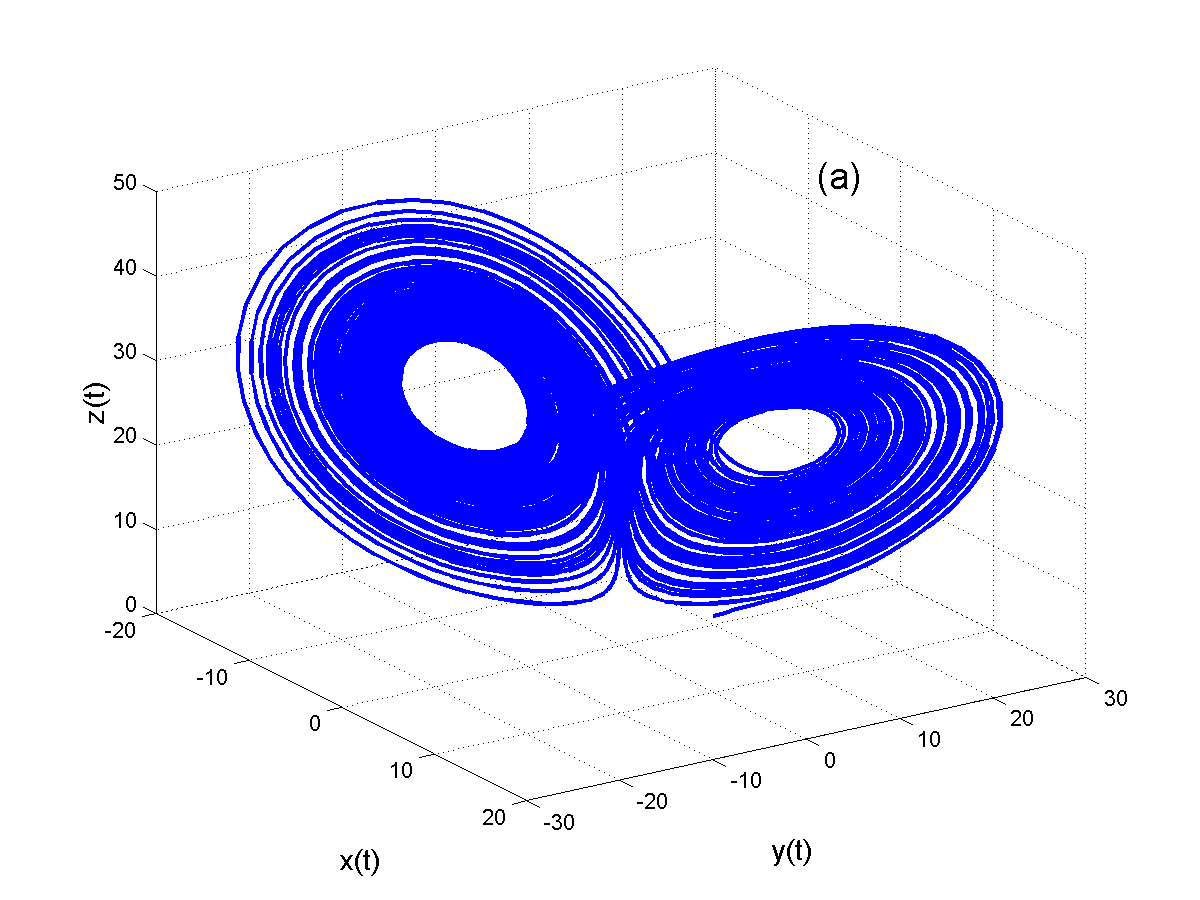
\includegraphics{Figuras/lorenzpack1.png}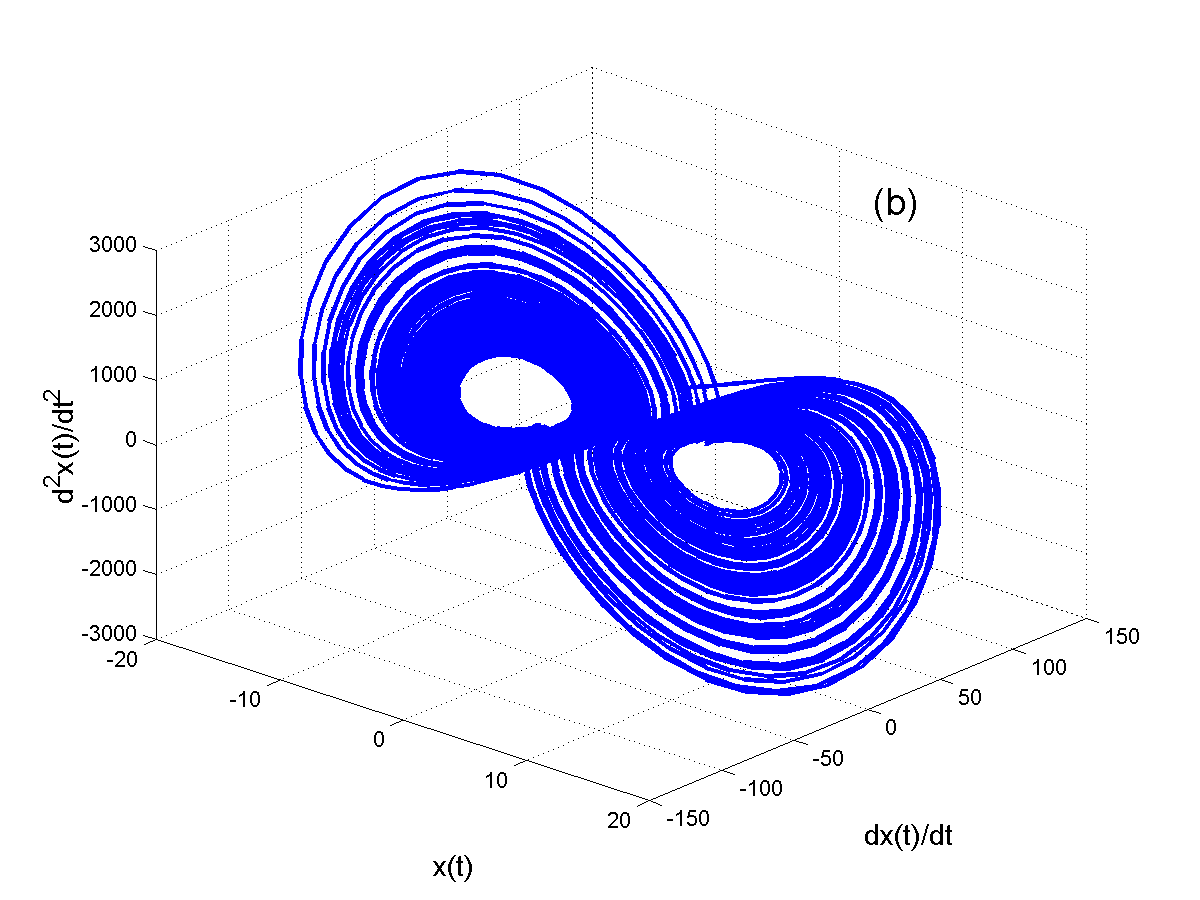
\includegraphics{Figuras/lorenzpack2.png}}
\caption{Atrator de Lorenz para o Sistema~(\ref{eqsistemalorenzpart}). (a) Atrator original. (b) Atrator reconstruído pelo método das derivadas.}
\label{lorenzdiff}
\end{figure}

As derivadas $dx/dt,d^{2}x/dt^{2}$ ou de ordens superiores podem ser aproximadas por equações de diferenças com passo pequeno. Assim:

\begin{equation}
\begin{array}{rcll} \dfrac{dx}{dt} & \simeq & \dfrac{x(t+h)-x(t)}{h} & h\rightarrow 0 \\ 
                     & & &  \\
                    \dfrac{d^{2}x}{dt^{2}} & \simeq & \dfrac{x(t+2h)-2x(t+h)+x(t)}{h^2} & h\rightarrow 0 
\end{array}
\label{eqderivadapack}
\end{equation}

A determinação numérica de derivadas a partir de um conjunto discreto de pontos é bastante sensível ao ruído, o que torna seu cálculo muito impreciso. Além disso, o passo $h$ possui um valor finito, de maneira que a qualidade da aproximação de uma derivada por uma equação de diferença diminui com o aumento da ordem da derivada~\cite{monteiro/02}. Desta forma, tal algoritmo torna-se pouco prático, principalmente se o número de variáveis de estado envolvido for grande.

Os problemas constatados com o método de \citeauthoronline{packard/80} são evitados utilizando-se um procedimento proposto por \citeonline{tak/81}. Takens provou que, no espaço de fase formado pelos eixos $x(t),x(t+\tau),x(t+2\tau),\ldots,x(t+(m-1)\tau)$, o atrator reconstruído é topologicamente equivalente ao atrator ``real'', sobre o qual conhece-se apenas a evolução em tempo discreto da variável de estado $x$. Na sua prova, Takens assumiu que a série é formada por infinitos pontos e que não há ruído. Segundo Takens, se essas condições são satisfeitas, as propriedades topológicas do atrator reconstruído são preservadas, e a reconstrução do mesmo é feita com base na relação:

\begin{equation}
m\geq 2D_{0}+1,
\label{eqconditak}
\end{equation}
onde $D_{0}$ é a dimensão de contagem de caixas do atrator associado.
 
Contudo, sua condição é suficiente mas não necessária, e, desta forma, a dimensão do atrator reconstruído pode obedecer a relação $m\geq D_{0}+1$ \cite{ding/93a}. Chama-se \textit{espaço de imersão} (``embedding space'') o espaço no qual realiza-se a reconstrução. Denomina-se $m$ de \textit{dimensão de imersão} (``embedding dimension'') e $\tau$ o \textit{passo da reconstrução} ou \textit{tempo de atraso} (``time delay''). Note que $\tau$ deve ser um múltiplo do espaçamento (ou tempo de amostragem) $\Delta t$ dos pontos da série temporal.

Pelo \textit{método dos atrasos temporais} de Takens, a cada instante $t_{i}$, assinala-se o ponto de coordenadas $x(t_{i}),x(t_{i}+\tau),\ldots,x(t_{i}+(m-1)\tau)$ no espaço de imersão. Variando-se $i$ de $1$ até $N$, obtém-se a trajetória reconstruída. Supondo que $\vec{\xi}_{\alpha}$ represente a posição do ponto no espaço de imersão no instante $t_{\alpha}$, a trajetória reconstruída é formada pela seqüência:

\begin{equation}
\vec{\xi}_{\alpha}=(x(t_{\alpha}),x(t_{\alpha}+\tau),x(t_{\alpha}+2\tau),...,x(t_{\alpha}+(m-1)\tau))
\label{eqtakensreconst}
\end{equation} 
com $\alpha=1,\ldots,M$. As constantes $m,\tau,N,M$ relacionam-se por $N=M+(m-1)\tau$. Assumindo que a série temporal é o resultado de um processo determinístico, cada $\vec{\xi}_{\alpha+1}$ é o resultado de um mapeamento desconhecido, $\mathcal M(\vec{\xi}_{\alpha})$, ou seja,

\begin{equation}
\vec{\xi}_{\alpha+1}=\mathcal M(\vec{\xi}_{\alpha})
\label{eqtakensreconst2}
\end{equation} 

\subsubsection{A escolha do passo}

\citeonline{tak/81} demonstrou que para um número infinito de pontos e na ausência de ruído a escolha do passo de reconstrução $\tau$ é na grande maioria dos casos arbitrária. Entretanto, as séries temporais experimentais são finitas, usualmente contaminadas com ruído externo e obtidas com o uso de filtros. Nessa situação, a reconstrução depende da escolha correta do passo. Se o passo $\tau$ for muito pequeno $x(t),x(t+\tau)$ e $x(t+2\tau)$, por exemplo, terão praticamente o mesmo valor\footnote{Admite-se que a freqüência de amostragem, relacionada com o intervalo de tempo $\Delta t$ entre duas medidas consecutivas, é suficientemente elevada para capturar toda a estrutura fina do sinal, ou seja, que ela seja adequada para se monitorar com detalhe a evolução temporal do sistema.}. Como conseqüência, o atrator reconstruído fica comprimido em torno da diagonal $z=y=x$, já que $\vec{\xi}_1\simeq\vec{\xi}_2\simeq\vec{\xi}_3$, ou seja, esse atrator apresentará uma dependência linear entre $\vec{\xi}_1,\vec{\xi}_2$ e $\vec{\xi}_3$, que não ocorre nas componentes reais $x,y$ e $z$ (conforme Figura~\ref{figlorenzpasso}(a)). Por outro lado, como a trajetória real está restrita a um volume finito do espaço de fase, o passo $\tau$ não pode ser muito grande, sob pena dos vetores reconstruídos $\vec{\xi}_i$ serem completamente não-correlacionados, cobrindo todo o espaço de fase (conforme Figura~\ref{figlorenzpasso}(c)).

\begin{figure}[ht]
\centering 
\resizebox{7.2cm}{!}{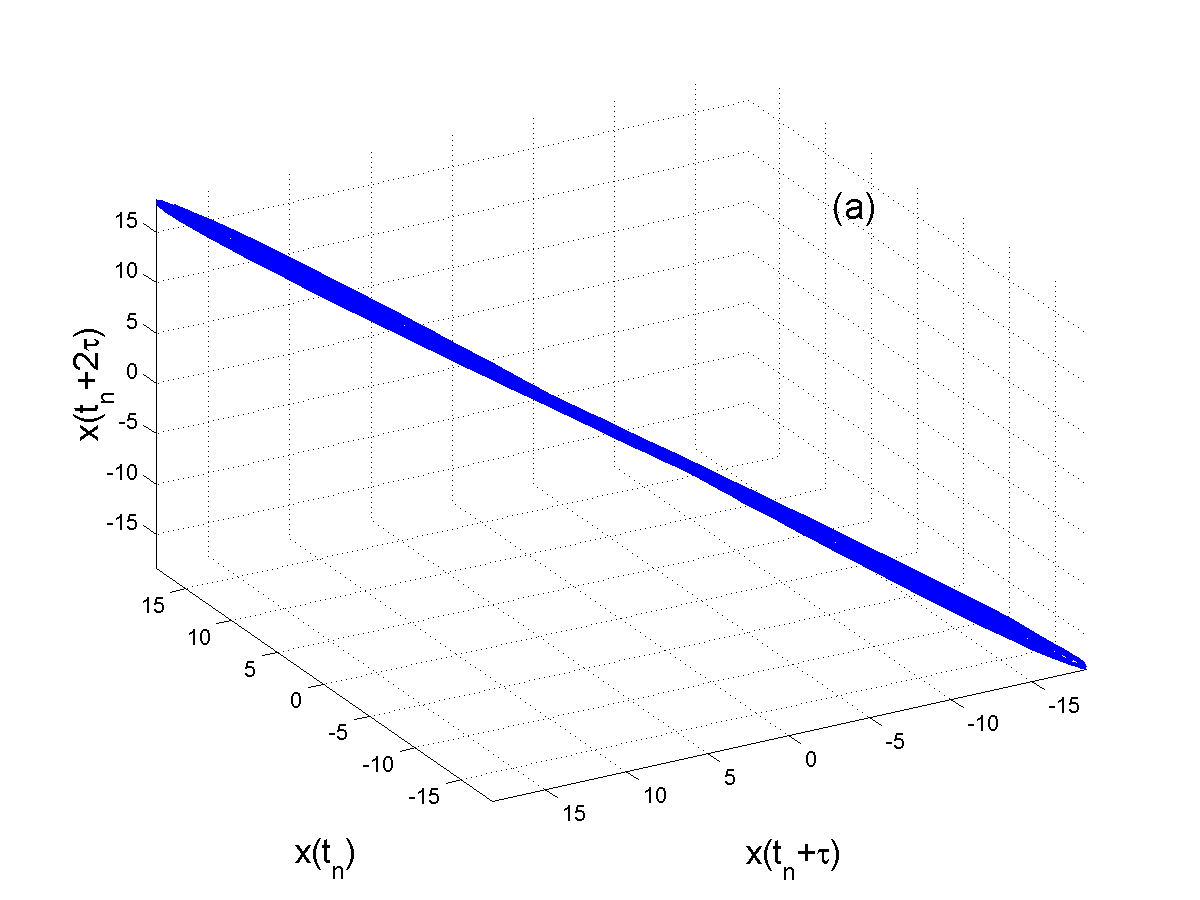
\includegraphics{Figuras/lorenzatraso1.png}} \resizebox{7.2cm}{!}{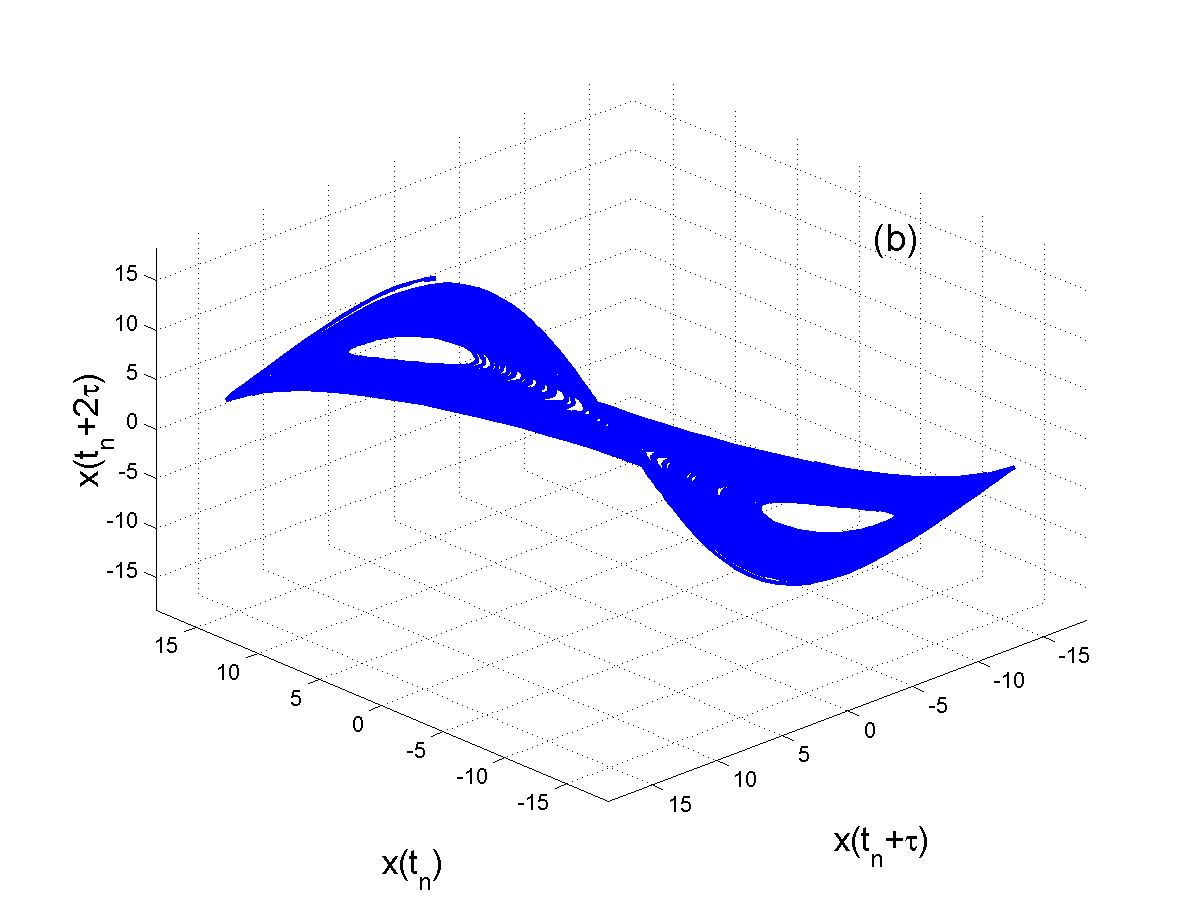
\includegraphics{Figuras/lorenzatraso2.png}} \\  \resizebox{7.2cm}{!}{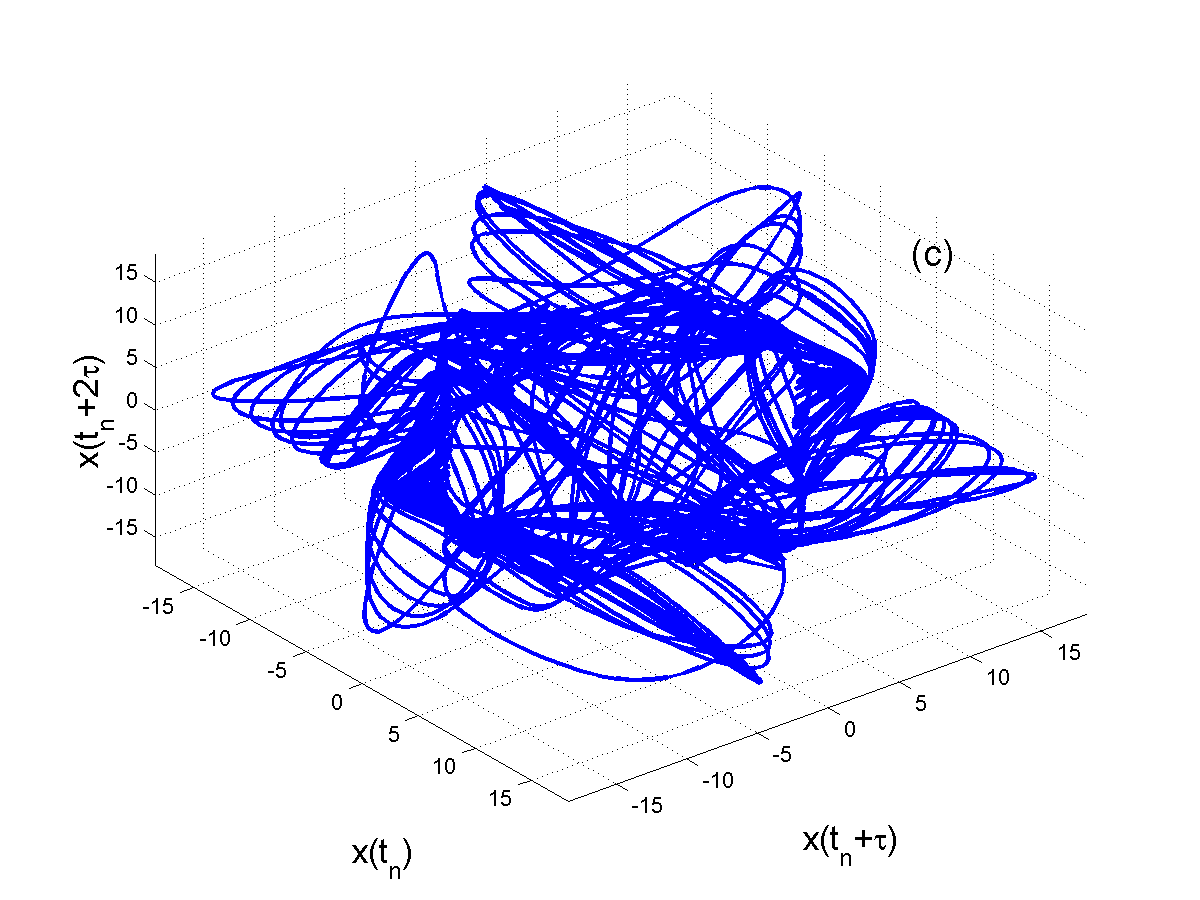
\includegraphics{Figuras/lorenzatraso3.png}} 
\caption{Exemplo da influência do passo na reconstrução do atrator de Lorenz associado ao Sistema~(\ref{eqsistemalorenzpart}). (a) passo muito pequeno ($\tau=1$). (b) passo adequado ($\tau=12$). (c) passo muito grande ($\tau=50$).}
\label{figlorenzpasso}
\end{figure}

Diversos trabalhos têm proposto critérios para orientar a escolha do passo correto~\cite{fraswi/86}. O critério mais difundido, e também utilizado nesta dissertação, consiste em examinar a correlação entre os pares de pontos em função de seu tempo de separação, ou seja, através da função de autocorrelação (já definida na Seção~\ref{secanalisetrad}). Após determinar o tempo do primeiro ``zero'' desta função, uma modesta fração deste valor é uma escolha razoável para o atraso $\tau$ \cite{gollub/98}.

A sensibilidade do processo de reconstrução relativamente ao passo pode ser estimada através de um método bastante prático e rápido: o chamado \textit{gráfico de primeiro retorno}, que consiste em graficar-se $x(t_{i})\times x(t_{i}+\tau)$, reconstruindo-se para tanto vetores bidimensionais com passo $\tau$ (conforme Figura~\ref{figlorenzprimeiroret}). Uma simples inspeção visual desse gráfico fornece informações sobre os valores de $\tau$ para os quais $x(t_{i})$ e $x(t_{i}+\tau)$ está ainda fortemente correlacionados, situação em que o atrator reconstruído fica comprimido próximo à diagonal e, desta forma, indica quão sensível é a reconstrução do atrator relativamente à escolha do passo, quão homogêneo é o atrator e qual o número típico de vetores reconstruídos necessário para caracterizá-lo completamente~\cite{monteiro/02}. 

\begin{figure}[ht]
\centering 
\resizebox{7.2cm}{!}{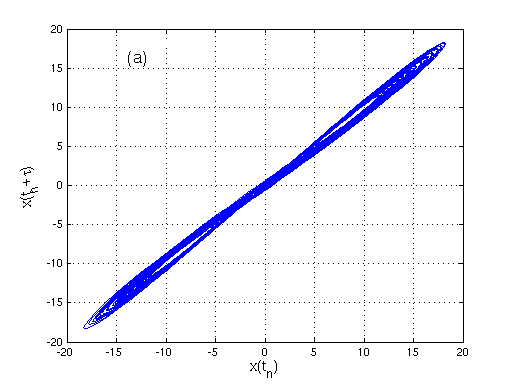
\includegraphics{Figuras/lorenzreconstbi1.png}} \resizebox{7.2cm}{!}{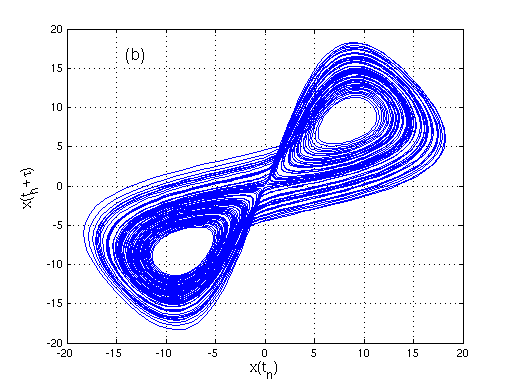
\includegraphics{Figuras/lorenzreconstbi12.png}} \\  \resizebox{7.2cm}{!}{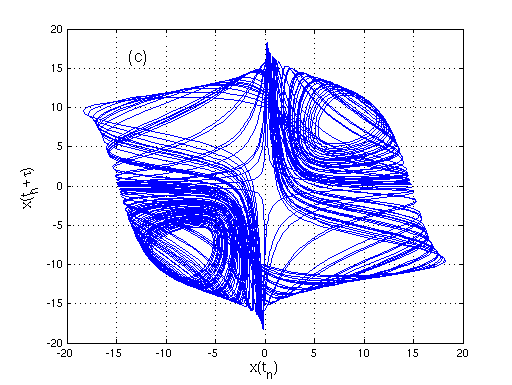
\includegraphics{Figuras/lorenzreconstbi50.png}} 
\caption{Gráfico de primeiro retorno a partir da variável $x$ que é parte da solução do Sistema~(\ref{eqsistemalorenzpart}). (a) $\tau=1$. (b) $\tau=12$. (c) $\tau=50$.}
\label{figlorenzprimeiroret}
\end{figure}

\subsubsection{A escolha da dimensão de imersão}
\label{secdimimers}

\paragraph*{Dimensões generalizadas}
Atratores caóticos apresentam um comportamento irregular e os mesmos não preenchem completamente o espaço de fase devido à contração do elemento de volume~\cite{argyris/94}. Um atrator caótico imerso em um espaço de fase tridimensional é uma forma ``híbrida'' entre uma superfície e um objeto espacial e assim sua dimensão está entre $2$ e $3$, ou seja, é um fractal. Desta forma, a caracterização desse atrator é realizada com base no conceito generalizado de dimensão que no caso de atratores regulares como pontos fixos, ciclos limites e toros, coincidem com a dimensão convencional em geometria euclidiana, ou seja, $0$, $1$ ou $2$.

Existe um conjunto infinito de dimensões, $D_{q}$, conhecidas como dimensões generalizadas, que definem propriedades métricas ou probabilísticas de um atrator~\cite{hentschel/83}. Deixe um atrator caótico ser coberto por $m(\varepsilon)$ quadrados de lado $\varepsilon$, e seja $M$ o número total de pontos observados no atrator. Então, a probabilidade de que um ponto se encontre no $i$-ésimo quadrado é obtido pela razão $p_{i}=M_{i}/M$, onde $M_{i}$ é o número de pontos do atrator que se encontra no $i$-ésimo quadrado. O conjunto infinito de dimensões generalizadas é dado por

\begin{equation}
D_{q}=\dfrac{1}{q-1}\lim_{\varepsilon\rightarrow\infty}\dfrac{\ln \sum_{i=1}^{m(\varepsilon)}p_{i}^q}{\ln \varepsilon}
\label{eqdimgeneral}
\end{equation}

onde $q$ está relacionado às possíveis definições da dimensão. Quando $q=0$, a relação~(\ref{eqdimgeneral}) produz simplesmente a dimensão de contagem de caixas $D_{0}$ sobre o atrator. A dimensão de informação $D_{1}$ e a dimensão de correlação $D_{2}$ são obtidas no limite da Equação~(\ref{eqdimgeneral}) quando $q$ tende para $1$ e $2$, respectivamente. $D_{1}$ pode ser expresso como~\cite{farmer/83}

\begin{equation}
D_{1}=\lim_{\varepsilon\rightarrow 0}\dfrac{\ln \sum_{i=1}^{m(\varepsilon)}p_{i} \ln p_{i}}{\ln \varepsilon}
\label{eqdiminfor}
\end{equation}

que é conhecida como dimensão de informação ou dimensão entrópica.

A dimensão de correlação, proposta por \citeonline{grassproca/83} como uma forma de caracterizar atratores caóticos, é dada pela relação

\begin{equation}
D_{2}=\lim_{r\rightarrow\ 0}\frac{\log C(r)}{\log r}
\label{eqcorr2}
\end{equation}
onde $C(r)$ é a função de correlação integral definida como

\begin{equation}
C(r)=\frac{1}{M^2}\sum_{i,j=1 \\, i\neq j}^{M} \Theta\left(r-\left \|\vec{\xi}_{i}-\vec{\xi}_{j}\right \|\right),
\label{eqcorr1}
\end{equation}
onde $M$ é o número de pontos no atrator, $\|\|$ denota a norma euclidiana que quantifica a distância entre os pares de vetores em espaços de imersão arbitrários e $\Theta(x)$ é uma função degrau de Heavyside, definida por
\begin{equation}
\Theta(x)=\
\left\{ \begin{array}{ccl}
 1,  &  \mathrm{se} & x\geq 0   \\
 0,  &  \mathrm{se} & x< 0
\end{array}
\right.  
\label{eqheavyside}
\end{equation}

A correlação integral (\ref{eqcorr1}) conta a freqüência relativa de pares cuja separação é menor que a escala $r$. Note que a Equação~(\ref{eqcorr2}) implica que para pequenos valores de $r$, a correlação integral $C(r)$ comporta-se como uma lei de potência $C(r)\approx r^{D_{2}}$. Conseqüentemente, o cálculo do expoente pode ser obtido a partir de um gráfico de $C(r)$ versus $r$ em escala $\log$-$\log$.

Para valores de $q\geq3$, \citeonline{hentschel/83} fornecem aproximações para as dimensões generalizadas $D_{3},D_{4},\ldots$ associando funções de correlação integral entre triplas, quádruplas, etc. de vetores. É possível mostrar que estas dimensões estão ordenadas da seguinte maneira: $D_{0}\geq D_{1}\ldots\geq D_{n}$, sendo que a igualdade é válida sob a hipótese de que os pontos do atrator sejam uniformemente distribuídos.

Em geral, o expoente $D_{2}$ é mais fácil de ser estimado que o expoente $D_{0}$ devido ao grande esforço computacional empregado na procura da dimensão de contagem de caixas~\cite{greenside/82}. Em diversos sistemas, a dimensão de contagem de caixas $D_{0}$ e a dimensão de correlação $D_{2}$ são muito próximas uma da outra e, desta maneira, o valor de $D_{2}$ fornece uma boa estimativa do número mínimo de equações diferenciais não-lineares necessárias para descrever o atrator~\cite{moon/97}.

% Na prática, para um conjunto finito de dados com resolução temporal discreta e finita exatidão, o limite em (\ref{eqcorr2}) pode não ser rigorosamente alcançado. Porém, em um gráfico de $\log C(r,M)$ versus $\log r$, uma parte linear aparece para valores intermediários de $r$. Sua inclinação fornece uma estimativa da dimensão de correlação \cite{rudolf/95}.

% Conforme a Figura~\ref{lorenzdiff}(a) o atrator de Lorenz cuja dimensão fractal é de aproximadamente $d=2.16$, pode ser bem representado em um espaço de imersão $m=3$. Contudo, em uma série temporal arbitrária a dimensão $d$ do atrator é desconhecida e, desta forma, o valor $m$ também o é. 

A implementação do algoritmo de Grassberger-Procaccia é relativamente simples. Entretanto, esse algoritmo  exige o cálculo e a classificação de aproximadamente $n(n-1)$ distâncias, onde $n$ é o número de vetores reconstruídos pela relação~(\ref{eqtakensreconst}). Este procedimento consome um tempo de processamento  excessivamente longo se o algoritmo não é construído  de forma otimizada, sobretudo se a série temporal for muito longa. Diversas sugestões, simplificações e modificações têm sido propostas~\cite{theiler/87,parker/89,malraison/83}. O procedimento adotado nesta dissertação reduz o cálculo de distâncias por considerar apenas um subconjunto de vetores reconstruídos, escolhidos de forma aleatória~\cite{malraison/83}. Como a escolha é aleatória, espera-se que o subconjunto de distâncias calculadas reproduza a estatística do conjunto de todas as distâncias, mantendo inalterado o valor de $C(r)$.

Na medida em que há limitações experimentais fortes para a obtenção de séries de dados longas, esse fato, aliado ao excessivo tempo de processamento, restringe a utilização do algoritmo de Grassberger-Procaccia para o caso de atratores de alta dimensão. Na grande maioria das aplicações a sinais experimentais, o algoritmo de Grassberger-Procaccia não permite estimar com segurança dimensões de correlações $D_{2}$ maiores de $4$ e $5$, as quais correspondem a dimensões de imersão da ordem de $9$ e $11$, respectivamente. 

A dimensão de correlação $D_{2}$ é uma das principais ferramentas usadas para identificar a existência de dinâmica caótica. Caos determinístico, em geral, é identificado se a inclinação de $C(r)$ versus $r$ converge para um valor de saturação, para valores cada vez mais altos da dimensão de imersão $m$ \cite{grassproca/83}. Em sinais determinísticos com comportamento caótico, o valor $D_{2}$ alcança um valor máximo devido a natureza de baixa dimensão do sistema. Desta forma, a dimensão de saturação obtida é uma aproximação para a dimensão fractal do atrator. A partir da relação~(\ref{eqconditak}), o valor da dimensão de imersão $m$ pode ser estimado. O valor desta dimensão permite ``desdobrar'' o atrator adequadamente, de modo que suas trajetórias não se cruzem no espaço de imersão. 

A Figura~\ref{figatratorhipot} ilustra o atrator de Lorenz imerso em espaços de fase de dimensões $2$ e $3$, respectivamente. A imersão no espaço de fase de duas dimensões dá origem a falsos cruzamentos das trajetórias (conforme Figura~\ref{figatratorhipot} (a)). Esses falsos cruzamentos podem estar ligados a falsos vizinhos próximos - um efeito que produz erros no cálculo do expoente de Lyapunov. Somente o espaço de fase tridimensional esboça este atrator completamente (conforme Figura~\ref{figatratorhipot} (b)). Este fato mostra a importância da imersão do atrator reconstruído em um espaço de fase adequado.

\begin{figure}[ht]
\centering 
\resizebox{15cm}{!}{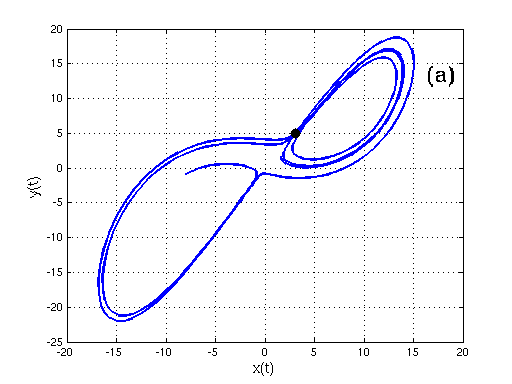
\includegraphics{Figuras/lorenzproj1.png}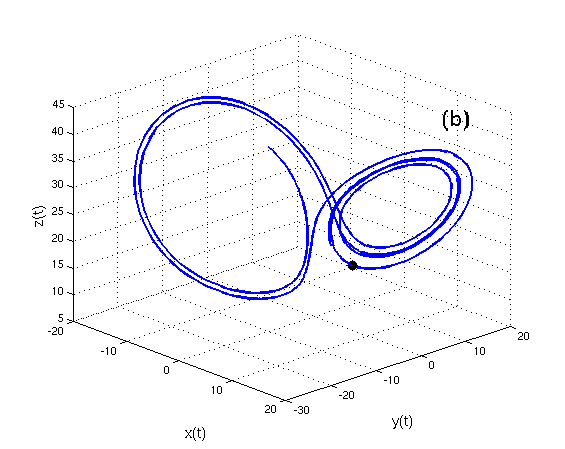
\includegraphics{Figuras/lorenzproj2.png}}
\caption{Efeito da imersão do atrator de Lorenz em espaços de diferentes dimensionalidades. (a) A imersão no espaço de fase bidimensional ocorre um falso cruzamento (marcado com um ponto em preto). (b) O atrator é completamente representado no espaço tridimensional.} 
\label{figatratorhipot}
\end{figure}

A Figura~\ref{figlorenzdimensoes}(b) mostra a correlação integral da série temporal em $x$ de Lorenz (Figura~\ref{figlorenzdimensoes}(a)) versus a escala $r$ em diferentes dimensões de imersão. Pode-se observar que cada uma destas curvas possui seções lineares, cujos valores das inclinações, calculados via regressão linear, saturam quando as dimensões de imersão são incrementadas. Estes valores de inclinações em função das dimensões de imersão que variam de $1$ a $10$ podem ser vistos através da Figura~\ref{figlorenzdimensoes}(c). Foram feitas $5$ realizações análogas à descrita acima, e a dimensão de correlação média obtida foi de $\langle D_{2}\rangle=2.105$ com desvio padrão de $\sigma_{D_{2}}=0.01$. Ainda, na Figura~\ref{figlorenzdimensoes}(c) pode ser observada a dimensão de correlação obtida a partir de uma série temporal aleatória (ruído branco). Para este caso, o valor de $D_{2}$ não satura quando as dimensões de imersão são incrementadas. Este comportamento já era esperado, pois um ruído branco está associado a um processo estocástico e não a uma dinâmica caótica.

\begin{figure}[ht]
\centering 
\resizebox{7.2cm}{!}{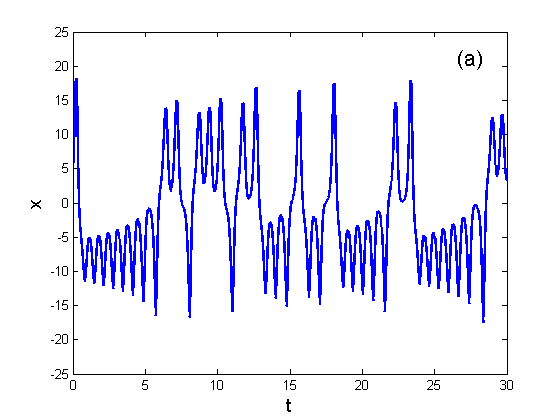
\includegraphics{Figuras/lorenzst.png}} \resizebox{7.2cm}{!}{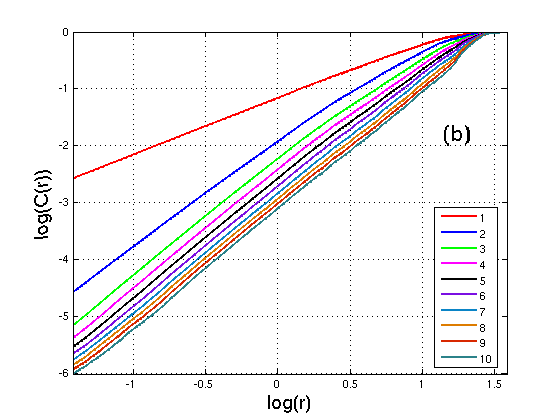
\includegraphics{Figuras/lorenzcorrelint2.png}} \\  \resizebox{7.2cm}{!}{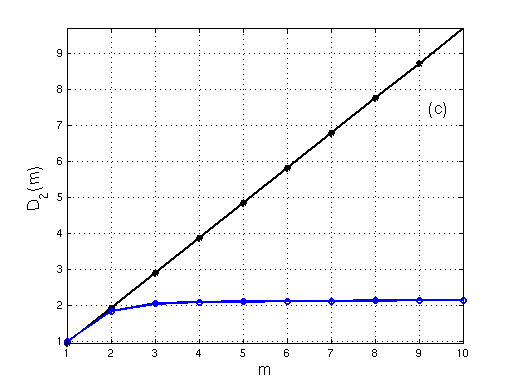
\includegraphics{Figuras/lorenzdimcorrel2.png}} 
\caption{(a) Série temporal obtida a partir da integração do Sistema~(\ref{eqsistemalorenzpart}). (b) Correlação integral da série em (a) com $m=1$ a $10$. (c) Dimensão de correlação de $D_{2}\langle2.105\rangle$ para a série de Lorenz (curva -o- em azul) e dimensão de correlação infinita para uma série aleatória (curva -*- em preto)}
\label{figlorenzdimensoes}
\end{figure}

\paragraph*{Distinção entre dinâmica de baixa dimensão e aleatoridade}

\citeonline{osboproven/89} oferecem um contra-exemplo da visão tradicional de que a inclinação de $C(r)$ versus $r$ aumenta continuamente para processos estocásticos, quando a dimensão de imersão $m$ é incrementada~\cite{grassproca/83}. Especificamente, tais autores mostraram que uma classe simples de ruído ``colorido'', caracterizado por uma lei de potência no espectro da forma $S(w)\approx w^{-\alpha}$ conduz à saturação em $D_{2}$ conforme a relação $D_{2}=2/(\alpha-1)$~\cite{osboproven/89,theilerj/91}. Este resultado tem sérias implicações sobre o estudo experimental de comportamento caótico determinístico, já que a observação de um valor finito de $D_{2}$ pode não ser suficiente para afirmar a presença de atratores caóticos em um sistema dinâmico. 

Em contrapartida, \citeonline{provenzalesmith/92} apresentam alguns testes que podem ser usados na distinção entre dinâmica de baixa dimensão e aleatoriedade em séries temporais. Esses testes são baseados na idéia de se modificar algumas propriedades de uma série temporal, com o intuito de verificar se a convergência de $D_{2}$ depende ou não dessas propriedades modificadas. 

O primeiro de tais testes é denominado ``teste surrogate'' e consiste em considerar a distribuição das fases de Fourier de uma série temporal. Desta forma, é aplicada a transformada de Fourier (conforme a Equação~(\ref{eqfourierdis})) na série em estudo. Em seguida, suas fases são embaralhadas uniformemente e é aplicada a transformada de Fourier inversa. A série temporal obtida com este processo é aleatória, já que o surrogate destrói as correlações existentes na série temporal que lhe deu origem, porém seu espectro de potência é similar ao da série original. Se a convergência de $D_{2}$ é determinada apenas pela forma do espectro (ou equivalentemente pela função de autocorrelação), então os resultados não são afetados pelo embaralhamento das fases. A invariância do valor de $D_{2}$ sobre as fases embaralhadas sugere fortemente que tais estimativas não indicam uma dinâmica caótica~\cite{provenzalesmith/92}. 

A Figura~\ref{figlorenzsurrogate}(a) mostra a série temporal obtida a partir do surrogate da série temporal em $x$ de Lorenz, a Figura~\ref{figlorenzsurrogate}(b) mostra a correlação integral obtida para dimensões de imersão que variam de $1$ a $10$ e finalmente a Figura~\ref{figlorenzsurrogate}(c) apresenta a dimensão de correlação, $D_{2}$, associada. A aparência da série temporal com surrogate é completamente diferente da apresentada na Figura~\ref{figlorenzdimensoes}(a) e os respectivos valores de $D_{2}$ são também bastante distintos (ver Figuras~\ref{figlorenzsurrogate}(c) e \ref{figlorenzdimensoes}(c)). Foram feitas $5$ realizações análogas à descrita acima, e pode-se observar que a dimensão de correlação $D_{2}$ em todos os casos não satura. Esse comportamento sugere fortemente a existência de uma dinâmica de baixa dimensão na série temporal de Lorenz. %Desta forma, em uma série temporal arbitrária, a constatação de um comportamento similar ao encontrado acima \textit{sugere} fortemente a existência de um atrator caótico associado~\cite{provenzalesmith/92}. 

\begin{figure}[ht]
\centering 
\resizebox{7.2cm}{!}{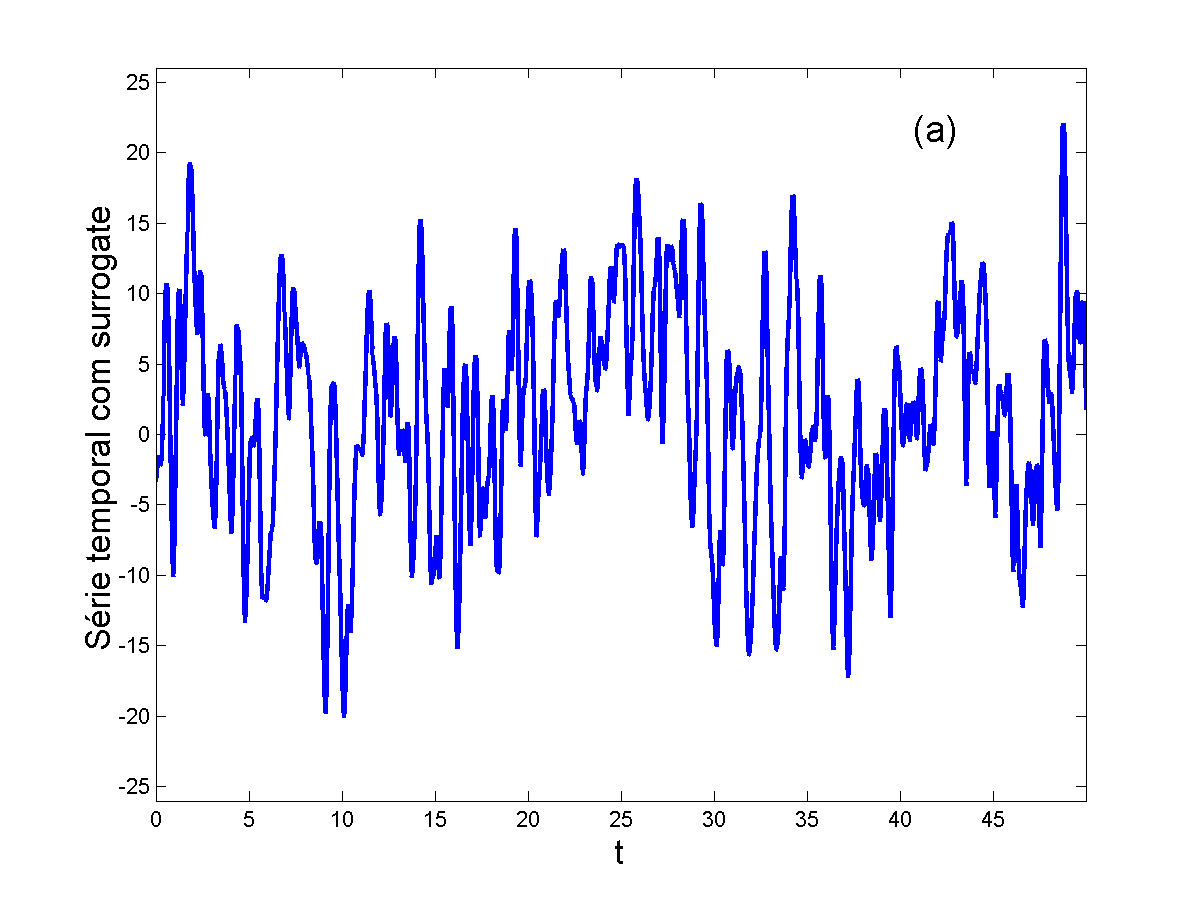
\includegraphics{Figuras/lorenzxsurr.png}} \resizebox{7.2cm}{!}{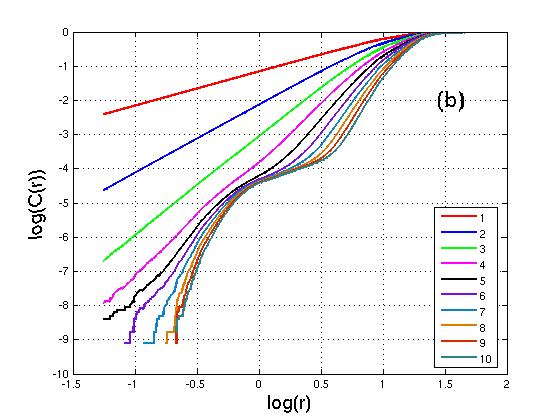
\includegraphics{Figuras/lorenzcorrelint2surr.png}} \\  \resizebox{7.2cm}{!}{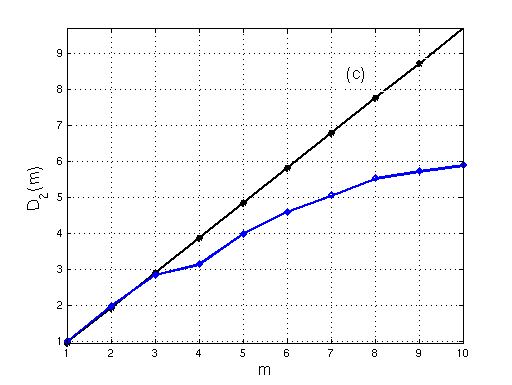
\includegraphics{Figuras/lorenzdimcorrelsurr2.png}} 
\caption{(a) Série temporal de Lorenz em $x$ com fase embaralhada. (b) Correlação integral da série em (a) com $m=1$ a $10$. (c) Dimensão de correlação da série em (a) e dimensão de correlação infinita para uma série aleatória}
\label{figlorenzsurrogate}
\end{figure}

Outro teste consiste em considerar a análise da correlação integral~(\ref{eqcorr1}) da primeira derivada numérica (ou primeira diferença) de uma série temporal. Para um sistema governado por um atrator caótico de baixa dimensão, o valor de $D_{2}$ é o mesmo tanto para a série temporal original quanto para série temporal modificada. Isto porque a primeira derivada numérica (ou primeira diferença) mantem as correlações existentes na série original. 

A Figura~\ref{figlorenzdiff}(a) apresenta a primeira diferença $\Delta x(t)=x(t+\Delta t)-x(t)$ da componente $x$ do atrator de Lorenz, a Figura~\ref{figlorenzdiff}(b) apresenta a correlação integral para $\Delta x$ e a Figura~\ref{figlorenzdiff}(c) apresenta os valores de $D_{2}$ associados. Foram feitas $5$ realizações análogas à descrita acima, e a dimensão de correlação média obtida foi de $D_{2}=\langle2.09\rangle$ com desvio padrão de $\sigma_{D_{2}}=0.03$. Pode-se observar, neste caso, que a dimensão de correlação $D_{2}$ satura em um valor bastante próximo daquela obtido com base na série original. Este comportamento sugere mais uma vez a existência de uma dinâmica de baixa dimensão na série temporal de Lorenz. Ainda, como $D_{2}\thickapprox 2.09$, pela relação de Takens dada por~(\ref{eqconditak}), o atrator de Lorenz pode ser bem representado em um espaço de imersão de $m=6$.

\begin{figure}[ht]
\centering 
\resizebox{7.2cm}{!}{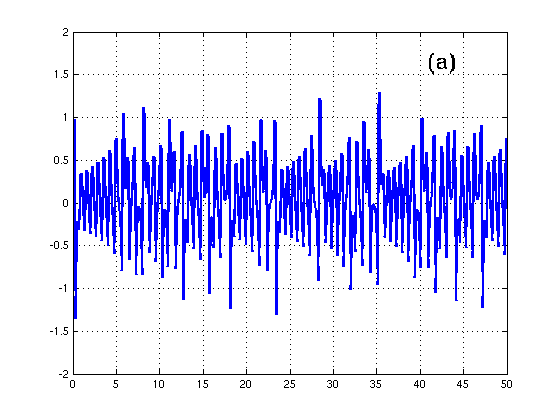
\includegraphics{Figuras/lorenzdiff2.png}} \resizebox{7.2cm}{!}{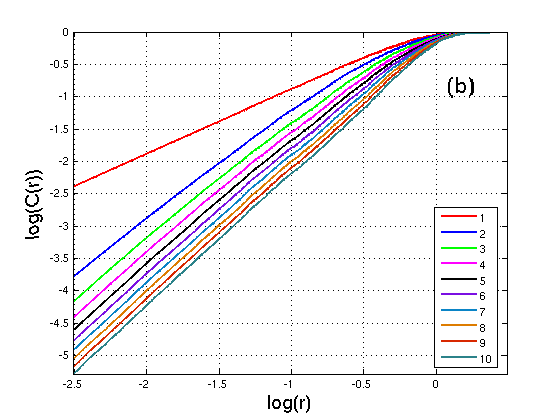
\includegraphics{Figuras/lorenzcorrelintdiff2.png}} \\  \resizebox{7.2cm}{!}{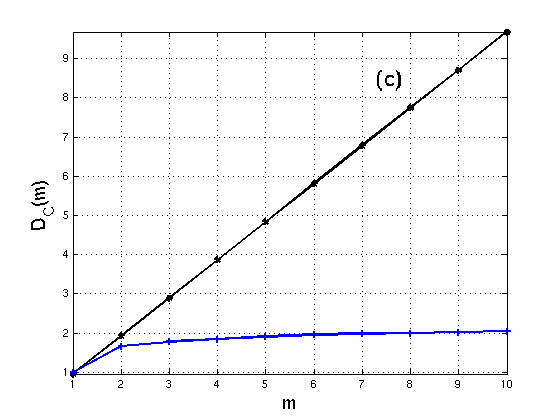
\includegraphics{Figuras/lorenzdimcorreldiff2.png}} 
\caption{(a) Série temporal gerada a partir da primeira diferença da série temporal $x$ de Lorenz. (b) Correlação integral da série em (a) com $m=1$ a $10$. (c) Dimensão de correlação da série em (a) e dimensão de correlação infinita para uma série aleatória.}
\label{figlorenzdiff}
\end{figure}

A técnica de reconstrução do espaço de fase (\ref{eqtakensreconst}) como também o cálculo da dimensão de correlação (\ref{eqcorr2}) devem ser usados após uma avaliação cuidadosa das condições de sua aplicabilidade, seguida de uma avaliação da consistência dos resultados obtidos. Uma aplicação ingênua de tais métodos pode levar a conclusões errôneas~\cite{osboproven/89}. \citeonline{eckruelllyap/92} fornecem evidências segundo as quais o valor de $D_{2}$, estimado a partir do algoritmo de Grassberger-Procaccia, não fornece dimensões confiáveis maiores que:

\begin{equation}
D_{2_{\textrm{max}}}=2\log_{10}N
\label{eqlimitemax}
\end{equation}
onde $N$ é o número de pontos da série temporal. Desta forma, quando o valor da dimensão de correlação satura em um valor superior ao estabelecido pela Equação~(\ref{eqlimitemax}) pode não ser correto afirmar a série temporal possui uma dinâmica de baixa dimensão. Sob essa perspectiva, a dimensão de correlação obtida a partir de $10.000$ pontos da série em $x$ de Lorenz é confiável já que seu valor, a saber $D_{2}\thickapprox 2.1$, satisfaz a relação $D_{2_{\textrm{max}}}\leq 8$.

\subsubsection{Estacionaridade}
\label{subsecestacio}

O estudo das propriedades de um atrator associado a um sistema dinâmico 
admite que o mesmo se encontre em um \textit{estado estacionário}\footnote{Sob o ponto de vista estatístico, uma série temporal é estacionária se a função de densidade de probabilidade associada não se altera ao longo do tempo (estacionaridade plena), ou particularmente se os primeiros momentos associados a uma série temporal, como média e variância não se alteram ao longo do tempo (estacionaridade estrita).}, ou para o caso de um experimento real, muito próximo desse estado - situação em que os pontos representativos da evolução temporal do sistema estão bastante próximos do atrator associado à dinâmica. Desta forma, é importante verificar se a série temporal em estudo corresponde, de fato, a um estado estacionário do sistema físico real~\cite{aguirre/00}.

O critério de estacionaridade utilizada nesta dissertação emprega janelas de dados deslizantes ao longo de uma série. Ou seja, dada uma série temporal~(\ref{eqserietemp}), pode-se definir como janelas de dados deslizantes todos os subconjuntos de amostras subseqüentes possíveis, de comprimento $L$ (conforme Figura~\ref{figestaciogeral}). Testes que envolvem tais janelas procuram analisar e quantificar as propriedades que se alteram ao longo da série temporal, como a média e a variância, com base em um determinado intervalo de confiança~\cite{alvaro/01}.

% \begin{figure}[ht]
% \centering \resizebox{15cm}{!}{\includegraphics{Figuras/figestacionaria.png}}
% \caption{Janelas de dados deslizantes} 
% \FONTE{\cite{alvaro/01}}
% \label{figestaciogeral}
% \end{figure}

\begin{figure}[!ht]
\begin{center}
\resizebox{12cm}{!}{\input{Figuras/estacionariaxfig2.pdftex_t}}
\caption{Janelas de dados deslizantes} 
\end{center}
\label{figestaciogeral}
\end{figure}
 
Desta forma, médias parciais ($\mu_{\textrm{parcial}}$) e variâncias parciais ($\sigma_{\textrm{parcial}}$) devem satisfazer as relações:
\begin{equation}
\begin{array}{rcccl}
\mu_{\textrm{total}}-\sigma_{\textrm{total}} & \leq  &  \mu_{\textrm{parcial}} & \leq  & \mu_{\textrm{total}}+\sigma_{\textrm{total}}\\
&   &   &   &\\
\sigma_{\textrm{total}}^2-\sigma_{\textrm{total}} & \leq  &  \sigma_{\textrm{parcial}}^2 & \leq  & \sigma_{\textrm{total}}^2+\sigma_{\textrm{total}}
\end{array}
\label{eqestacionaria}
\end{equation} 
onde $\mu_{\textrm{total}}$, $\sigma_{\textrm{total}}$ e $\sigma_{\textrm{total}}^2$ são a média, desvio padrão e variância da série temporal, respectivamente.

O teste de estacionaridade descrito acima foi aplicado à série $x$ de Lorenz com janelas deslizantes de comprimento $L=100$. Como todos os valores parciais de $\mu$ e $\sigma$ satisfazem a relação~(\ref{eqestacionaria}) pode-se dizer que tal série é estacionária.


\subsubsection{Os expoentes de Lyapunov}

Em séries temporais experimentais, o ponto de partida para o cálculo dos expoentes de Lyapunov é o atrator reconstruído em uma dimensão de imersão $m$ adequada. Uma vez reconstruído o atrator, define-se uma trajetória de referência (ou trajetória fiducial) a partir da seqüência de vetores reconstruídos. Em seguida, deve-se analisar o que ocorre com pontos vizinhos desta trajetória. Com as informações sobre as taxas de divergência destes pontos, pode-se obter, então, os expoentes de Lyapunov. 

Diversos métodos têm sido propostos para estimar esses expoentes em séries temporais experimentais~\cite{wolf/85,eckrue/86,sanosawada/85}. O método proposto por \citeonline{wolf/85} permite calcular com expressiva precisão o maior expoente de Lyapunov (positivo). Considere uma trajetória descrita pela seqüência de pontos $y(t_0), y(t_1), y(t_2),\cdots$ no atrator reconstruído. Seja $z_0(t_0)$ o vizinho no atrator reconstruído mais próximo de $y(t_0)$ e $L_0$ a distância entre $y(t_0)$ e $z_0(t_0)$ (conforme Figura~\ref{figferraralyap}), isto é, $L_0=\left|y(t_0)-z_0(t_0)\right|<\epsilon$, e desta forma, $z_0(t_0)$ está dentro da hiperesfera de raio $\epsilon$ centrada em $y(t_0)$. Acompanha-se então a evolução temporal de $z_0$ e $y_0$ até que num instante $t_1$ a distância entre esses pontos, $L_0{'}$, exceda $\epsilon$. Nesse momento substitui-se $z_0$ por um novo vizinho, mais próximo de $y(t_1)$, que esteja na direção do segmento $L_0{'}$ e tal que $L_1=\left|y(t_1)-z_1(t_1)\right|<\epsilon$. O processo prossegue até que todos os pontos $y(t_i)$ tenham sido percorridos. O maior expoente de Lyapunov positivo é obtido como a média de $\log_{2} L_i{'}/L_i$, ao longo da trajetória de referência, isto é,

\begin{equation}
\lambda_{1}=\frac{1}{t_{M}-t_{0}}\sum_{i=0}^{M-1}\log_{2}\frac{L_i{'}}{L_i}
\label{lyap2}
\end{equation}
onde $M$ é o número total de vezes que um novo vizinho foi escolhido próximo à trajetória de referência.

\begin{figure}[ht]
\centering \resizebox{13cm}{!}{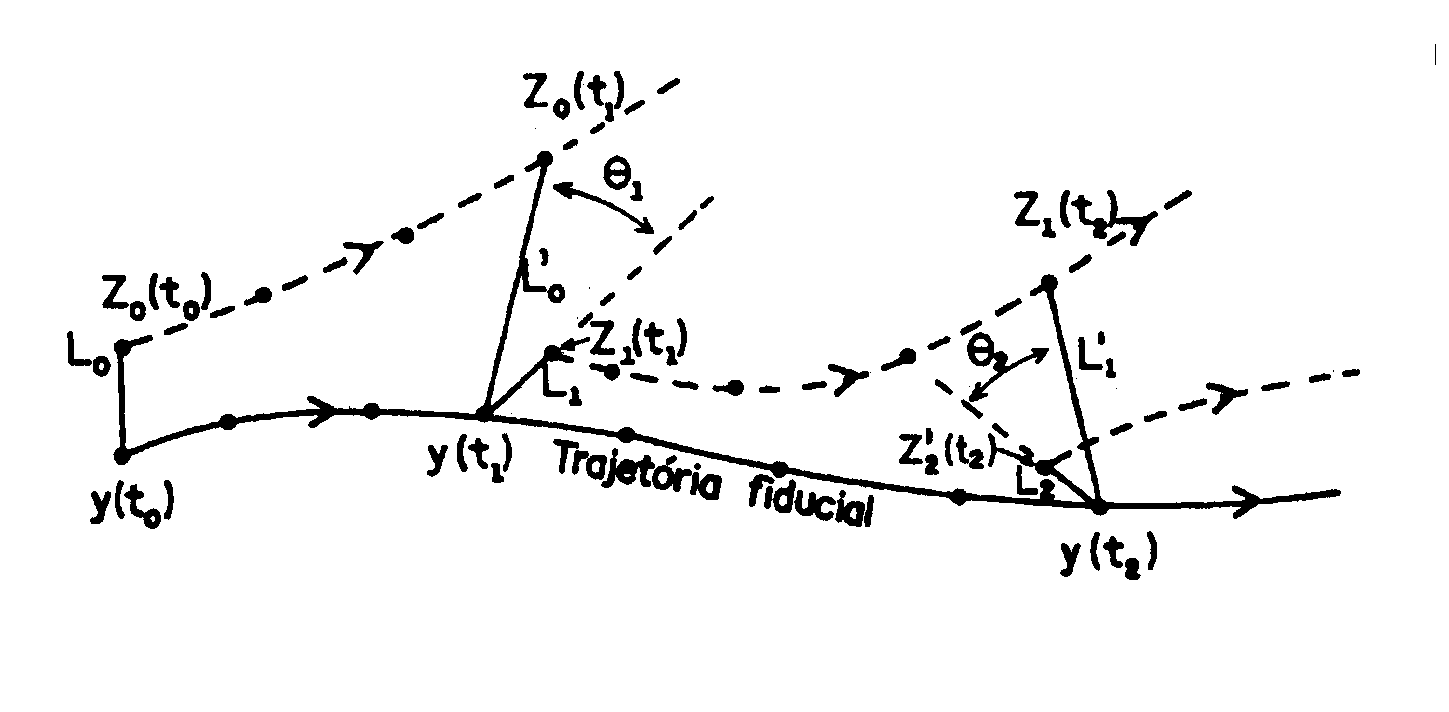
\includegraphics{Figuras/wolf.png}}
\caption{Representação esquemática do método proposto por \citeonline{wolf/85}. O maior expoente de Lyapunov é estimado a partir da taxa de crescimento dos segmentos $L_i$. Quando o comprimento do segmento que liga dois pontos próximos do atrator excede um certo valor $\epsilon$, um novo vizinho é escolhido de forma a minimizar o ângulo $\theta_i$.}
\FONTE{Adaptada de \citeonline{wolf/85}}
\label{figferraralyap}
\end{figure}

Através do método descrito acima é possível obter uma aproximação numérica para o maior expoente de Lyapunov, $\lambda_1$, calculado a partir da série temporal em $x$ de Lorenz. Pode-se observar que a aproximação obtida é satisfatória já que o maior expoente de Lyapunov, obtido diretamente do Sistema de EDO's (\ref{eqsistemalorenz}) é aproximadamente $2.16$ \cite{wolf/85}, enquanto que o obtido com base no algoritmo de \citeonline{wolf/85} é $2.18\pm0.01$.

\begin{figure}[ht]
\centering \resizebox{13cm}{!}{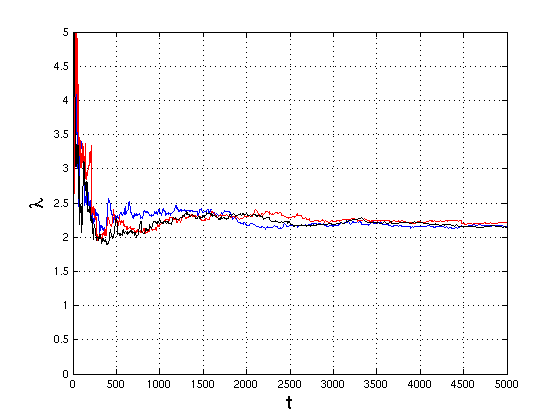
\includegraphics{Figuras/lorenzlyap3cond.png}}
\caption{Convergência do maior expoente de Lyapunov ($\lambda_1$) associado à componente $x$ do atrator de Lorenz, com base no algoritmo desenvolvido por \citeonline{wolf/85}. A curva azul corresponde à condição inicial $(5,5,5)$, a curva vermelha corresponde à condição inicial $(5.01,5,5)$ e a curva preta corresponde à condição inicial $(5,10,5)$}
\label{figlorenzlyap}
\end{figure}

\subsection{Plots de Recorrência}

A representação gráfica bidimensional de uma matriz da forma:

\begin{equation}
R_{i,j}=\Theta(\varepsilon-\|\xi_{i}-\xi_{j}\|),\;\;\; i,j=1,\ldots,M
\label{eqplotrec}
\end{equation}

é definida como \textit{Plots de Recorrência} (PR) e foi introduzida por \citeonline{eckmannplotrecorr/87}. Desta forma, $\xi_{i}\in\mathds{R}^m$ são vetores de dimensão $m$ obtidos através da reconstrução do espaço de fase (\ref{eqtakensreconst}), $\varepsilon$ é um valor limite pré-definido e $\Theta$ é uma função degrau de Heavyside (conforme~\ref{eqheavyside}). Se a distância entre dois vetores $\xi_{i}$ e $\xi_{j}$ sobre a trajetória reconstruída for menor que $\varepsilon$, a função de Heavyside $\Theta$ assume o valor $1$, e neste caso a posição $(i,j)$ da matriz~(\ref{eqplotrec}) é representada por um ponto preto, caso contrário tal posição é representada por um ponto branco~\cite{eckmannplotrecorr/87,thielromano/04,thielemuitos/02,gaocai/00}.

Segundo \citeonline{eckmannplotrecorr/87} por meio de um PR é possível visualizar o comportamento de trajetórias no espaço de fase~\cite{eckmannplotrecorr/87} e ainda um PR mostra todos os tempos no qual um estado de um sistema dinâmico se repete. A repetição de estados é uma propriedade fundamental de um sistema dinâmico determinístico, e é um comportamento típico em sistemas caóticos ou não-lineares~\cite{thieltese/04}. 

Tradicionalmente, a visualização de espaços de fase com dimensões maiores que $3$ é feita por meio de projeções em sub-espaços de dimensão $2$ ou $3$. Contudo, um PR permite investigar a evolução de trajetórias em um espaço de fase com dimensões elevadas por meio da representação bidimensional de suas repetições. 

A Figura~\ref{figrpsistemas} apresenta PRs para um sistema estocástico, um sistema periódico e um sistema determinístico caótico. PRs associados à sistemas estocásticos freqüentemente apresentam uma certa homogeneidade em relação à distribuição de seus pontos (conforme Figura~\ref{figrpsistemas}(a)). Sistemas que oscilam periódicamente apresentam estruturas de repetições periódicas cujas distâncias entre esses padrões periódicos correspondem ao período (conforme Figura~\ref{figrpsistemas}(b)). Sistemas dinâmicos caóticos possuem estruturas diagonais paralelas à diagonal principal (conforme Figura~\ref{figrpsistemas}(c)). Essas estruturas ocorrem quando um segmento da trajetória reconstruída é paralelo à outro segmento, ou seja, a trajetória visita a mesma região do espaço de fase em diferentes tempos. O comprimento de tais estruturas é proporcional à duração da evolução local comum entre os segmentos da trajetória~\cite{thieltese/04,gaocai/00}.

\begin{figure}[ht]
\centering 
\resizebox{7.2cm}{!}{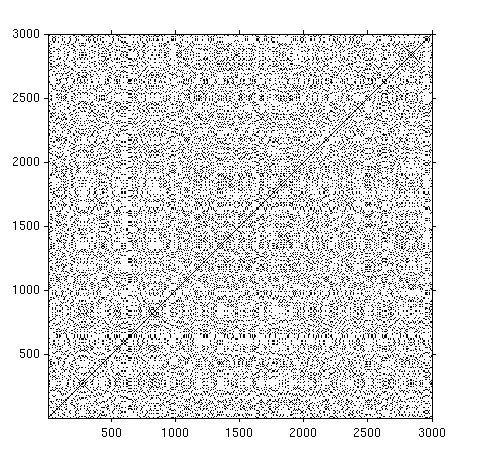
\includegraphics{Figuras/ruidorp.png}} \resizebox{7.2cm}{!}{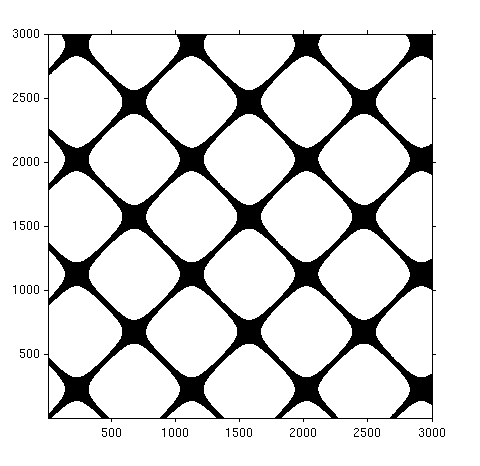
\includegraphics{Figuras/senorp.png}} \\  \resizebox{7.2cm}{!}{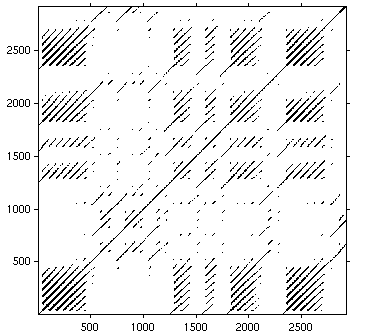
\includegraphics{Figuras/lorenzrp.png}} 
\caption{(a) PR para um sistema estocástico (ruído uniformemente distribuído) com $m=1$ e $\varepsilon=0.09994$ . (b) PR para a função seno com $m=1$ e $\varepsilon=0.2$. (c) PR correspondente à componente em $x$ do atrator de Lorenz com $m=6$ e $\varepsilon=4.9344$. O valor de $\varepsilon$ utilizados nos casos (a) e (b) correspondem à $10\%$ das variâncias associadas, e no caso (c) à $10\%$ do diâmetro do espaço de fase~\cite{thielromano/04}.}
\label{figrpsistemas}
\end{figure}

% \begin{figure}[ht]
% \centering 
% \resizebox{13cm}{!}{\includegraphics{Figuras/lorenzdet.png}\includegraphics{Figuras/lorenzembardet.png}}
% \caption{Atrator de Lorenz para o sistema~(\ref{eqsistemalorenzpart}). (a) Atrator original. (b) Atrator reconstruído pelo método das derivadas.}
% \label{lorenzdiff}
% \end{figure}

Uma das principais vantagens na aplicação de um PR, em comparação à aplicação de técnicas de caracterização de comportamento caótico tradicionais (como por exemplo o algoritmo de Grassberger e Procaccia~(\ref{eqcorr2})), é que o PR pode ser aplicado em séries temporais não estacionárias e com poucos pontos~\cite{thieltese/04}. Uma desvantagem é que se o número de pontos da série temporal for muito grande (maior que 10.000 pontos), o número de vetores reconstruídos é também grande. Conseqüentemente, a ordem da matriz de distâncias~(\ref{eqplotrec}) se torna elevada. Este fato pode acarretar em insuficiência de memória computacional na armazenagem desta matriz.



